% ======================================================================
% paper.tex
% From Natural Language to Verifiable Reasoning:
% A Semantic Reduction Framework for Reliable AI Mathematics
%
% Compile (paper is self-contained; all figures are drawn with TikZ):
%   pdflatex paper
%   bibtex   paper
%   pdflatex paper
%   pdflatex paper
% or: latexmk -pdf paper.tex
% ======================================================================
\documentclass[11pt,a4paper]{article}

% ---------- Encoding & fonts ----------
\usepackage[T1]{fontenc}
\usepackage[utf8]{inputenc}
\usepackage{newtxtext}             % Times-like text
\usepackage[margin=1in]{geometry}

% ---------- Math ----------
% amsmath/amsthm before newtxmath; newtxmath provides the AMS symbols,
% so amssymb is intentionally not loaded (avoids \Bbbk clash);
% option [amsthm] prevents the \openbox clash.
\usepackage{amsmath,amsthm}
\usepackage[amsthm]{newtxmath}
\usepackage{mathtools}

% ---------- Tables, figures, color ----------
\usepackage{booktabs}
\usepackage{multirow}
\usepackage{array}
\usepackage{xcolor}
\usepackage{caption}
\captionsetup{font=small,labelfont=bf}
\usepackage{enumitem}

% ---------- TikZ figures ----------
\usepackage{tikz}
\usetikzlibrary{positioning,arrows.meta,fit,backgrounds,calc}

% ---------- References ----------
\usepackage[round,sort&compress]{natbib}
\bibliographystyle{plainnat}

% ---------- Links (loaded last) ----------
\usepackage[colorlinks=true,linkcolor=teal!60!black,citecolor=teal!60!black,
            urlcolor=teal!60!black]{hyperref}

% ---------- Small utilities ----------
\usepackage{xspace}
\newcommand{\ir}{\textsc{ir}\xspace}
\newcommand{\kernel}{\mathcal{K}}
\newcommand{\reducemap}{\rho}
\newcommand{\rendermap}{r}
\newcommand{\policy}{g_\theta}
\newcommand{\artifact}[1]{{\ttfamily\scriptsize #1}}

% ---------- Theorem-like environments ----------
\theoremstyle{plain}
\newtheorem{proposition}{Proposition}
\newtheorem{observation}{Observation}
\theoremstyle{definition}
\newtheorem{definition}{Definition}
\newtheorem{example}{Example}
\theoremstyle{remark}
\newtheorem*{remark}{Remark}

\title{\bfseries From Natural Language to Verifiable Reasoning:\\
       A Semantic Reduction Framework for Reliable AI Mathematics}

\author{%
  Anonymous Author(s)\\
  \small C2 Challenge Submission --- replace with name and affiliation for camera-ready\\
  \small \texttt{anonymous@example.com}
}
\date{\today}

\begin{document}
\maketitle

% ======================================================================
\begin{abstract}
Large language models (LLMs) now produce fluent, apparently rigorous
solutions to mathematical problems, yet they continue to output
\emph{plausible but invalid} proofs: a natural-language argument cannot be
checked against a fixed formal semantics, so a mistaken step is
indistinguishable from a correct one without re-doing the reasoning. The
field has answered this reliability problem with three families of
techniques: search with verification, formalized proof, and reproducible
benchmarking. This paper argues that these answers share an overlooked
structural feature. We decompose an AI-for-mathematics (\textsc{ai4math})
system into three layers---\emph{generation}, \emph{semantic reduction},
and \emph{verification}---and show that the reduction map from informal
language to a computable, typed object is the decisive reliability
bottleneck: when this map fails, the verifier has no object to inspect and
hallucinations cannot, in principle, be detected; when it succeeds,
verification is deterministic and can be made sound. On this basis we
propose (i) a typed intermediate representation (\ir) in which natural
language serves only as an interface and the \ir\ as the execution core,
(ii) a generate$\to$\ir$\to$verify$\to$render pipeline with bidirectional
consistency between text and structure, and (iii) a concrete ten-item
reliability checklist for \textsc{ai4math} systems. A small, fully
reproducible reference implementation on a controlled word-problem
dialect instantiates the framework: across 36 problem instances the
verifiability rate was $0.833$, every failure localized at the reduction
layer, and kernel decisions on all 90 verifiable candidates were correct.
We state explicitly what these results do and do not establish, and
discuss applications to automated theorem proving, problem solving, and
assessment.
\end{abstract}

% ======================================================================
\section{Introduction}\label{sec:intro}

\subsection{Background}
Mathematics has become a flagship domain for modern AI. Systems built on
large language models solve a large fraction of grade-school and
competition problems on standard benchmarks such as \textsc{gsm8k}
\citep{cobbe2021gsm8k} and \textsc{math} \citep{hendrycks2021math}, while
specialized systems have reached olympiad-level performance in geometry
\citep{trinh2024alphageometry,chervonyi2025alphageometry2} and in formal
reasoning \citep{hubert2025alphaproof}. Two technical moves drive this
progress: eliciting intermediate reasoning steps through chain-of-thought
prompting \citep{wei2022cot}, and delegating parts of the computation to
external tools or programs \citep{chen2023pot,schick2023toolformer}.

This success, however, coexists with a characteristic failure mode. An LLM
emits a proof that \emph{reads} as correct---every sentence is plausible,
the notation is well formed, and the final answer may even be right---but
contains an invalid inference hidden in the middle. Such failures are not
rare anecdotes: performance varies sharply across numerically different
instantiations of the \emph{same} problem template, degrades as the number
of clauses grows, and can collapse when a single irrelevant clause is added
\citep{mirzadeh2024gsmsymbolic}. Fluent text, in other words, is weak
evidence of a valid argument.

\subsection{The reliability problem}
We call the central question the \emph{reliability problem}:
\begin{quote}
\itshape Given an AI-produced mathematical argument, can an external party
establish---without re-deriving the result---whether every inference is
valid, and can that establishment be repeated by anyone else?
\end{quote}
The literature offers three responses. \textbf{Search plus verification}:
sample many candidate solutions and rank them with a learned or
rule-based verifier \citep{cobbe2021gsm8k,wang2023selfconsistency,
lightman2024verify}. \textbf{Formalized proof}: express the problem in a
proof assistant such as Lean and have a small trusted kernel check the
proof object \citep{polu2020gptf,first2023baldur,xin2024deepseekprover,
hubert2025alphaproof}. \textbf{Reproducible evaluation}: pin down data,
prompts, seeds, and templates so that reported numbers can be regenerated
\citep{zheng2022minif2f,yang2023leandojo,mirzadeh2024gsmsymbolic}.

These responses are usually presented as alternatives. We instead read
them as instances of one underlying requirement: somewhere between the
model and the checker, informal language must be converted into a
\emph{computable object with a fixed meaning}. This paper makes that
conversion---which we term \emph{semantic reduction}---explicit, studies
where it fails, and builds a framework around it.

\subsection{Thesis and contributions}
Our thesis is:
\begin{quote}
\bfseries Reliability in \textsc{ai4math} cannot be obtained by final
verification alone, because verification can only inspect what reduction
has already made into an object. Semantic reduction must therefore be a
first-class, typed, and measurable system component.
\end{quote}

We make four contributions, of which the last three are deliberately small
and concrete:
\begin{enumerate}[leftmargin=2em,itemsep=2pt]
\item \textbf{A three-layer decomposition} (generation, semantic
reduction, verification) that reorganizes existing techniques and
localizes the dominant failure mode (\S\ref{sec:layers}--\S\ref{sec:bottleneck}).
\item \textbf{A typed-\ir\ framework}: a pipeline architecture in which
natural language is only an interface, together with a bidirectional
consistency requirement between text and structure (\S\ref{sec:framework}).
\item \textbf{A ten-item reliability checklist} that operationalizes the
framework for practitioners and reviewers (\S\ref{sec:checklist}).
\item \textbf{A reproducible reference implementation and case study}
that tests the central claim on a controlled dialect
(\S\ref{sec:casestudy}); code and pinned seeds are included.
\end{enumerate}

\subsection{Scope and outline}
The emphasis is on the structure of reliable systems and on AI-assisted
scholarship, not on deep new mathematics. We do \emph{not} claim that all
informal reasoning can or should be formalized, nor that the small case
study predicts benchmark performance; these boundaries are stated where
the relevant claims are made. \S\ref{sec:layers} defines the layers,
\S\ref{sec:bottleneck} analyzes reduction as the bottleneck,
\S\ref{sec:framework} presents the framework and checklist,
\S\ref{sec:related} reviews related work, \S\ref{sec:applications} gives
applications, and \S\ref{sec:discussion} discusses limitations and
extensions before \S\ref{sec:conclusion} concludes.

% ======================================================================
\section{A Three-Layer Decomposition}\label{sec:layers}

We model any \textsc{ai4math} system as the composition of three layers,
depicted in Figure~\ref{fig:layers}. Each layer has a different artifact,
a different notion of correctness, and a different failure structure.

\begin{figure}[t]
\centering
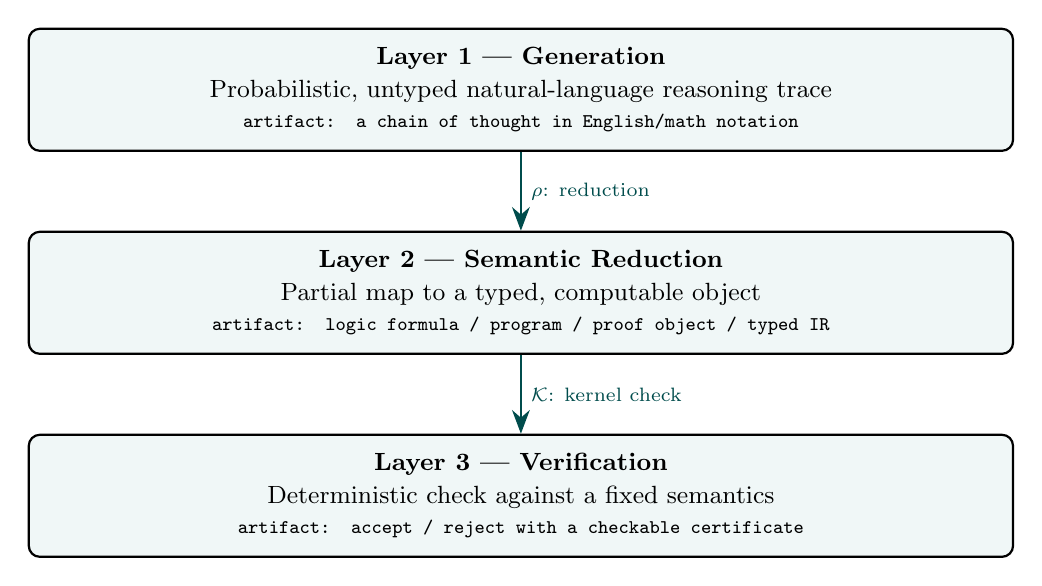
\begin{tikzpicture}[
  font=\small,
  layer/.style={draw,rounded corners,line width=.8pt,minimum width=12.5cm,
                minimum height=1.55cm,align=center,fill=teal!6},
  arrow/.style={-{Stealth[length=3mm]},thick,teal!60!black}]
\node[layer] (g) {\textbf{Layer 1 --- Generation}\\[.3mm]
  Probabilistic, untyped natural-language reasoning trace\\
  \artifact{artifact: a chain of thought in English/math notation}};
\node[layer,below=10mm of g] (s) {\textbf{Layer 2 --- Semantic Reduction}\\[.3mm]
  Partial map to a typed, computable object\\
  \artifact{artifact: logic formula / program / proof object / typed IR}};
\node[layer,below=10mm of s] (v) {\textbf{Layer 3 --- Verification}\\[.3mm]
  Deterministic check against a fixed semantics\\
  \artifact{artifact: accept / reject with a checkable certificate}};
\draw[arrow] (g) -- node[right,font=\scriptsize]{$\reducemap$: reduction} (s);
\draw[arrow] (s) -- node[right,font=\scriptsize]{$\kernel$: kernel check} (v);
\end{tikzpicture}
\caption{The three-layer decomposition. Generation produces informal text;
semantic reduction converts it to a typed object; verification checks that
object. The two arrows are qualitatively different maps: the first is
partial and meaning-sensitive, the second deterministic and mechanizable.}
\label{fig:layers}
\end{figure}

\subsection{Layer 1: Generation}
The generation layer maps a problem $q$ to a natural-language reasoning
trace $t$:
\begin{equation}
\policy : q \;\longmapsto\; t = (s_1,s_2,\dots,s_k),
\end{equation}
where each $s_i$ is a sentence mixing prose and notation. This is what
chain-of-thought prompting elicits \citep{wei2022cot}, and what
Minerva-style models produce at scale \citep{lewkowycz2022minerva}. Three
properties matter here. The map is \emph{probabilistic}: re-prompting
yields different traces. It is \emph{untyped}: sentences carry no machine
checkable declaration of what kind of object each symbol denotes. And it is
\emph{semantically open}: phrases such as ``it follows that'' or
``obviously'' do not specify which rule was applied or which prior
statements license the step. These properties make generation flexible but
leave validity as a property a human reader must judge.

\subsection{Layer 2: Semantic reduction}
The reduction layer attempts to attach a precise meaning to the trace by
mapping it into a formal, computable representation:
\begin{equation}
\reducemap : t \;\rightharpoonup\; i,
\end{equation}
where $i$ is a typed object and the harpoon denotes that the map is
\emph{partial}: it is undefined for text it cannot interpret. Concretely,
reduction targets one of four forms:
\begin{itemize}[leftmargin=2em,itemsep=2pt,topsep=3pt]
\item a \textbf{logical formula} in first- or higher-order logic;
\item an \textbf{executable program} in a programming language or DSL;
\item a \textbf{proof object} (a term of a proof assistant's type theory,
or a sequence of tactics);
\item a \textbf{typed intermediate representation} such as an annotated
AST or constraint graph.
\end{itemize}
The theoretical foundation for proof objects is the \emph{Curry--Howard}
correspondence, under which propositions are types and proofs are
inhabiting terms \citep{sorensen2006curryhoward}. Program-of-thoughts
prompting reduces to executable programs \citep{chen2023pot};
autoformalization reduces natural-language statements to Lean or Isabelle
terms \citep{polu2022curriculum,xin2024deepseekprover}; the DSL used by
AlphaGeometry is a domain-specific typed representation
\citep{trinh2024alphageometry}.

\subsection{Layer 3: Verification}
The verification layer checks the reduced object against a fixed formal
system, rather than against prose. Writing $\Gamma$ for the context of
axioms, definitions, and established lemmas and $\varphi$ for the target
proposition, the kernel decides a judgment
\begin{equation}
\Gamma \;\vdash\; i : \varphi ,
\end{equation}
returning accept or reject together with a certificate that can be
independently replayed. Depending on the object, the check establishes
\emph{derivability} (a theorem follows from the context),
\emph{consistency} (no contradictory constraints), \emph{factual
grounding} (referenced premises exist and are applied correctly), or
\emph{constraint satisfaction} (the computed value meets the target).
Tools include proof assistants with small trusted kernels---Lean
\citep{demoura2021lean4}, Coq, Agda, Isabelle---and SMT or symbolic
solvers. The defining property is that a sound kernel never accepts an
invalid object \emph{of the kind it claims to check}.

\begin{table}[t]
\centering
\caption{Taxonomy of reduction targets. Each target licenses a different
verification guarantee and is exemplified by a cited system.}
\label{tab:taxonomy}
\small
\begin{tabular}{@{}llll@{}}
\toprule
\textbf{Reduction target} & \textbf{Formal basis} & \textbf{Guarantee established} & \textbf{Example systems}\\
\midrule
Logical formula (FOL/HOL) & proof theory & logical consequence & SMT solvers, ATP\\
Executable program & operational/denot.\ semantics & computed value or property &
  PoT \citep{chen2023pot}, code tools\\
Proof object / tactics & Curry--Howard & theorem derivability &
  GPT-f \citep{polu2020gptf}, Baldur \citep{first2023baldur}\\
 & & & DeepSeek-Prover \citep{xin2024deepseekprover},
  AlphaProof \citep{hubert2025alphaproof}\\
Typed AST / DSL & type systems & well-typedness + constraints &
  AlphaGeometry \citep{trinh2024alphageometry}\\
Constraint graph & CSP semantics & feasibility & symbolic solvers\\
\bottomrule
\end{tabular}
\end{table}

\subsection{The two arrows are not symmetric}
The decomposition's content lies in the difference between its two arrows
(Table~\ref{tab:taxonomy}). The reduction arrow $\reducemap$ is partial,
meaning-sensitive, and as hard as translation: ambiguity in the source can
make multiple objects plausible. The verification arrow $\kernel$, by
contrast, is a total mechanized decision over well-formed inputs---it is
exactly the part that has been engineered to be trustworthy. A system that
speaks only of ``end-to-end verification'' conflates the two and thereby
hides where reliability is actually won or lost.

% ======================================================================
\section{The Bottleneck Is Semantic Reduction}\label{sec:bottleneck}

\subsection{What the verifier actually consumes}
A verifier cannot reach back into natural language. It consumes a
\emph{computable object}: a term to type-check, a program to run, a
constraint set to solve. Hence verification can establish validity only
conditional on reduction having built the right object:
\begin{proposition}[Conditional soundness]\label{prop:conditional}
Let $\kernel$ be a sound kernel and let $i=\reducemap(t)$. Then
\begin{equation}
\kernel\text{ accepts } i \ \wedge\ i\text{ faithfully encodes }t
\quad\Longrightarrow\quad t\text{ is a valid argument.}
\end{equation}
If reduction either fails or produces an object that does not encode the
intended argument, acceptance of $i$ implies nothing about $t$.
\end{proposition}
The second conjunct is usually left implicit---and is where the danger is.
A formal proof of the \emph{wrong statement} is still a valid proof
object; the kernel has done its job while the overall conclusion is false.

\subsection{Failure modes at the reduction layer}
We distinguish three recurrent reduction failures.
\begin{description}[leftmargin=2.2em,itemsep=2pt,topsep=3pt]
\item[Ambiguity (semantic instability).] The text admits more than one
formal reading. ``The product of consecutive numbers exceeds their sum by
one'' leaves the number of terms and the comparison implicit; different
reductions yield different formulas, and the model may silently pick one.
\item[Missing typing.] Symbols are introduced without a sort---a quantity
versus an index, a scalar versus a function, an integer versus a set. A
proof step that treats a length as an angle then has no well-typed target.
\item[Non-invertibility and free variables.] The text refers to quantities
never given (``some apples'', ``an unspecified price''). The resulting term
contains free variables and is not a closed object; no ground truth can be
computed, so the map is undefined.
\end{description}
These are precisely the failures our reference implementation makes
observable (\S\ref{sec:casestudy}).

\subsection{An event model of (un)reliability}
To make the bottleneck measurable, define four events for a produced
answer:
\begin{align}
R &= \{\text{reduction succeeds: a well-typed object exists}\},\\
F &= \{\text{the reduced object is faithful to the intended argument}\},\\
A &= \{\text{the kernel accepts the object}\},\\
T &= \{\text{the delivered conclusion is true}\}.
\end{align}
A sound kernel satisfies $A\wedge F \Rightarrow T$
(Proposition~\ref{prop:conditional}). Two consequences follow.
\emph{False acceptance}---a delivered conclusion the system certified---can
occur only when $A\wedge\neg F$: the kernel verified an unfaithful object.
\emph{Undetected error} occurs when $\neg R$: no object exists, so no
certificate of any kind is possible and a hallucination is outside the
verifier's reach. Conditioning on acceptance,
\begin{equation}
\Pr[T\mid A] = \Pr[F\mid A],
\end{equation}
because under a sound kernel acceptance guarantees truth exactly when the
object was faithful. Reliability engineering beyond the kernel is
therefore engineering of the event $F$---the quality of reduction---and of
the coverage of $R$. This motivates two metrics:
\begin{align}
\text{Verifiability rate}\quad V &= \Pr[R],\\
\text{False-acceptance rate}\quad \mathit{FA} &= \Pr[\neg T\mid A].
\end{align}
Reporting accuracy without $V$ is incomplete: an accurate answer that no
one can verify contributes nothing to reliability, and a high $V$ with low
faithfulness is actively dangerous.

\subsection{Why statistical verifiers do not close the gap}
Learned verifiers---outcome models that judge the final answer and process
models that score each step \citep{uesato2022process,lightman2024verify}---
improve accuracy and are cheap at inference. They do not, however,
implement Layer~3 as defined here. They return a calibrated probability
over correctness rather than a judgment against a fixed semantics, they are
themselves probabilistic and trained on the same distribution that
produces the errors, and they can share the generator's blind spots (for
instance, pattern-matching an off-by-one answer that ``looks right'').
Self-consistency \citep{wang2023selfconsistency} has the same status:
agreement across samples is evidence, not a certificate. These methods are
best understood as \emph{guides for search and reduction}---they decide
where a formal object is worth constructing---not as substitutes for the
kernel.

% ======================================================================
\section{The Framework}\label{sec:framework}

\subsection{A typed intermediate representation}
We propose making the reduction artifact explicit as a typed intermediate
representation with four components:
\begin{enumerate}[leftmargin=2em,itemsep=2pt,topsep=3pt]
\item a \textbf{type system} declaring the sort of every sub-object
($\mathrm{Int}$, $\mathrm{Rat}$, $\mathrm{Set}[\alpha]$,
$\mathrm{Func}[\alpha,\beta]$, $\mathrm{Proof}[\varphi]$, \dots);
\item an \textbf{operational semantics} fixing how objects evaluate or
reduce, so two implementations cannot disagree;
\item a \textbf{constraint system} carrying side conditions (domains,
ranges, well-definedness such as nonzero divisors);
\item a \textbf{compositional structure} (AST or graph) in which sub-proofs
and sub-computations are independently addressable and reusable.
\end{enumerate}
The type system is the key discipline: an ill-typed reduction is rejected
\emph{before} verification, converting silent semantic errors into visible
type errors. This is the same mechanism that makes proof assistants
trustworthy, applied at the reduction boundary.

\subsection{The generate--\ir--verify--render pipeline}
\begin{figure}[t]
\centering
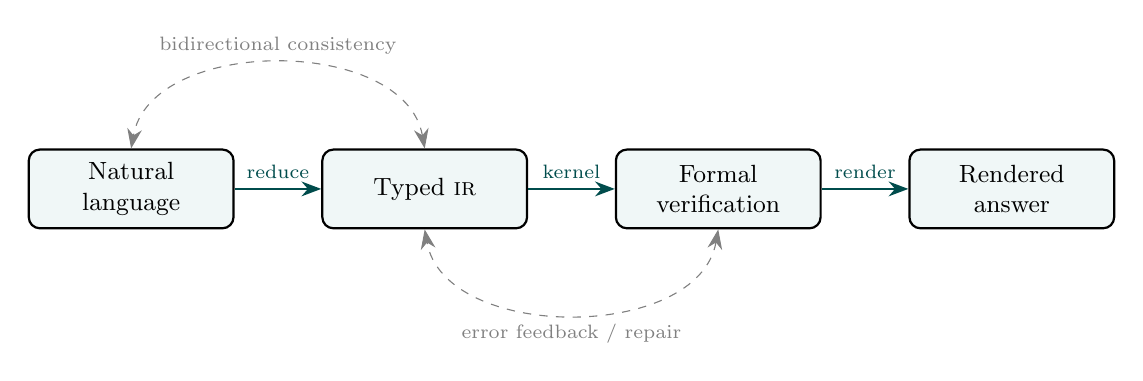
\begin{tikzpicture}[
  font=\small,node distance=8mm and 11mm,
  box/.style={draw,rounded corners,line width=.8pt,align=center,minimum height=10mm,
              minimum width=26mm,fill=teal!6},
  fwd/.style={-{Stealth[length=2.5mm]},thick,teal!60!black},
  fb/.style={{Stealth[length=2.5mm]}-{Stealth[length=2.5mm]},dashed,gray}]
\node[box] (nl) {Natural\\language};
\node[box,right=of nl] (ir) {Typed \ir};
\node[box,right=of ir] (ver) {Formal\\verification};
\node[box,right=of ver] (out) {Rendered\\answer};
\draw[fwd] (nl) -- node[above,font=\scriptsize]{reduce} (ir);
\draw[fwd] (ir) -- node[above,font=\scriptsize]{kernel} (ver);
\draw[fwd] (ver) -- node[above,font=\scriptsize]{render} (out);
\draw[fb] (ver.south) to[out=-100,in=-80]
  node[below,font=\scriptsize]{error feedback / repair} (ir.south);
\draw[fb] (ir.north) to[out=100,in=80]
  node[above,font=\scriptsize]{bidirectional consistency} (nl.north);
\end{tikzpicture}
\caption{The proposed pipeline. Natural language is the interface; the
typed \ir\ is the execution core. Rejection produces machine-readable
error feedback that drives repair, and every repaired object is
re-verified from scratch rather than patched around.}
\label{fig:pipeline}
\end{figure}

The standard workflow is:
\begin{equation}
\text{Natural language} \;\xrightarrow{\;\reducemap\;}\; \text{Typed \ir}
\;\xrightarrow{\;\kernel\;}\; \text{Verification}
\;\xrightarrow{\;\rendermap\;}\; \text{Rendered answer}.
\end{equation}
The key idea is a strict division of labor: prose is generated and rendered
for human communication, but all claims \emph{live} as \ir\ objects, and
only kernel-accepted objects are rendered as conclusions. Crucially,
rejection is not a dead end. The kernel emits a precise error (a type
mismatch, an unresolved premise, a failed constraint) that is fed back to
the generator; this is the mechanism shown effective by proof repair in
Baldur \citep{first2023baldur} and by tactic feedback in provers
\citep{xin2024deepseekprover}. Every repaired object is re-verified
\emph{from scratch}, so a repair cannot mask an earlier error.

\subsection{Bidirectional consistency}\label{sec:bidir}
Reduction has a companion rendering map $\rendermap: i\mapsto t'$ that turns
a verified object back into prose. We require a round-trip condition:
\begin{equation}
\rendermap(\reducemap(t)) \;\equiv\; t ,
\end{equation}
where $\equiv$ denotes semantic equivalence of the text, not literal
equality. This serves two purposes. \emph{Interpretability}: a reader can
inspect, for every formal step, the prose it corresponds to.
\emph{Traceability}: if the rendered text does not match what was said,
reduction silently changed the claim---the $\neg F$ event---and the
mismatch is caught by a human at the boundary rather than discovered after
a false acceptance. Bidirectional links are thus the practical instrument
for guarding faithfulness, which the kernel alone cannot check.

\subsection{A reliability checklist for \textsc{ai4math} systems}\label{sec:checklist}
As a directly usable contribution, Table~\ref{tab:checklist} distills the
framework into ten checks. It is written so that a reviewer can audit a
submission item by item; a system that cannot satisfy an item should say so
explicitly rather than leave the gap implicit.

\begin{table}[t]
\centering
\caption{A ten-item reliability checklist, organized by layer. Items are
binary and auditable; ``not applicable'' answers require justification.}
\label{tab:checklist}
\small
\begin{tabular}{@{}clp{8.6cm}@{}}
\toprule
\textbf{Layer} & \textbf{\#} & \textbf{Check}\\
\midrule
\multirow{2}{*}{Generation}
 & 1 & Problems, prompts, exemplars, and model versions are archived and versioned.\\
 & 2 & Multiple samples are drawn; disagreement or self-inconsistency is flagged, not averaged away.\\
\multirow{3}{*}{Reduction}
 & 3 & Every claim is mapped to a typed object with a declared signature.\\
 & 4 & Partial reductions are explicitly marked ``unverified''; no silent defaults or coercions.\\
 & 5 & Round-trip rendering is checked against the source text (\S\ref{sec:bidir}).\\
\multirow{3}{*}{Verification}
 & 6 & Objects are checked by a fixed, version-pinned, sound kernel.\\
 & 7 & The complete object is checked, not only the final answer; all premises are resolved.\\
 & 8 & Kernel errors drive repair; repaired objects are re-verified from scratch.\\
\multirow{2}{*}{Evaluation}
 & 9 & Verifiability rate $V$ is reported alongside accuracy, including robustness across template instantiations.\\
 & 10 & Code, seeds, \ir\ logs, and certificates are released so results can be regenerated.\\
\bottomrule
\end{tabular}
\end{table}

\subsection{Reproducible reference implementation and case study}\label{sec:casestudy}
To test the claim that failures localize at reduction, we include a small
reference implementation (\texttt{artifacts/reduction\_case\_study.py},
standard library only, pinned random seed). The domain is a controlled
dialect of arithmetic word problems with three families: one-step additive,
two-step give-away/earn, and rate/ratio with an aggregate discount. Each
problem is reduced by an explicit parser to a typed AST
($\mathrm{Int}$-saturated $\mathrm{Num}$ and $\mathrm{BinOp}$ nodes),
symbolically evaluated, and then presented with three candidate answers---
one correct and two wrong, including an off-by-one candidate that a
statistical reader might accept. We additionally instantiate
\emph{malformed} variants containing unbounded quantities
(``some apples'') or free variables (``an unspecified price'').

\begin{table}[t]
\centering
\caption{Case study results from a real run (seed pinned; reproducible via
the included script). All failures appear in the reduction columns; the
kernel never erred on an object it could inspect.}
\label{tab:casestudy}
\small
\begin{tabular}{@{}lrrrrrr@{}}
\toprule
\textbf{Family} & \textbf{Inst.} & \textbf{Red.\,+} & \textbf{Red.\,$-$}
 & \textbf{Correct accepted} & \textbf{Wrong rejected} & \textbf{Unverifiable}\\
\midrule
F1 one-step   & 12 & 10 & 2 & 10 & 20 & 6\\
F2 two-step   & 12 & 10 & 2 & 10 & 20 & 6\\
F3 rate/ratio & 12 & 10 & 2 & 10 & 20 & 6\\
\midrule
Total         & 36 & 30 & 6 & 30 & 60 & 18\\
\bottomrule
\end{tabular}
\end{table}

Table~\ref{tab:casestudy} reports the actual output. Of 36 problem
instances, 30 reduced to closed typed objects and 6 did not; the
\emph{verifiability rate} was $V=30/36=0.833$. On the 90 verifiable
candidate answers (30 correct, 60 wrong), the kernel accepted every
correct answer and rejected every wrong one---including all off-by-one
candidates---a classification rate of $1.000$. The 18 candidates attached
to malformed problems were neither accepted nor rejected: with no object to
check, they were simply \emph{unverifiable}, the $\neg R$ regime.

\begin{observation}\label{obs:case}
In the controlled dialect, every observed failure (6/6 reduction failures,
18/18 unverifiable candidates) lies at Layer~2; Layer~3 made no errors on
its defined inputs and Layer~1 outputs were harmless once reduction pinned
their meaning.
\end{observation}

\paragraph{Boundaries of the evidence.}
This is a proof-of-concept on a templated dialect, not a benchmark result:
the parser is hand-written, the semantics are elementary integer
arithmetic, and candidate generation is simulated rather than produced by
an LLM. The experiment supports the structural claim---that given a
faithful reduction, verification is deterministic, and that without it no
verification is possible---but says nothing about how often contemporary
LLMs achieve faithful reduction at scale, which is an empirical question
for which \citep{mirzadeh2024gsmsymbolic} and formal proving results such
as \citep{hubert2025alphaproof} provide complementary evidence.

% ======================================================================
\section{Related Work}\label{sec:related}

\paragraph{Reasoning via prompting.}
Chain-of-thought prompting demonstrates that intermediate steps improve
reasoning and that the ability emerges at sufficient scale
\citep{wei2022cot}; self-consistency replaces greedy decoding with
marginalization over sampled paths \citep{wang2023selfconsistency}. These
methods operate entirely in Layer~1 and therefore inherit its unverifiability;
in our framing they shape the distribution of traces but produce no object
a kernel can check.

\paragraph{Tool use and program-based reasoning.}
Toolformer shows that models can self-supervise API calls
\citep{schick2023toolformer}; program-of-thoughts prompting moves
computation into an interpreter, with the LLM responsible only for the
program \citep{chen2023pot}; Minerva fine-tunes a large model on technical
content and formats steps in \LaTeX \citep{lewkowycz2022minerva}. These are
instances of reduction to \emph{executable programs} (row~2 of
Table~\ref{tab:taxonomy}). Our framework makes explicit what they assume
implicitly: the program, not the prose, is the claim, and the interpreter
plays the kernel for the computational fragment while the reasoning
connecting programs still needs its own reduction.

\paragraph{Statistical verification.}
Outcome and process supervision train verifiers on final results or
individual steps \citep{uesato2022process}; the process-supervised results
of \citet{lightman2024verify} show strong gains on \textsc{math}. As argued
in \S3.4, these are probabilistic oracles that guide search rather than
sound checkers; they fit most naturally \emph{inside} the pipeline as
proposals for what to reduce and verify formally.

\paragraph{Formal theorem proving with learned components.}
GPT-f trains a transformer on Metamath and contributed the first
deep-learning proofs accepted into a formal library
\citep{polu2020gptf}; expert iteration with statement curriculum learning
extends this to olympiad problems \citep{polu2022curriculum}, evaluated on
the cross-system miniF2F benchmark \citep{zheng2022minif2f}. Baldur
generates whole proofs and repairs them using the proof assistant's error
messages \citep{first2023baldur}; LEGO-Prover grows a library of verified,
retrievable skills and solves roughly half of miniF2F test
\citep{wang2024lego}; LeanDojo provides open tooling, fine-grained premise
annotations, and a retrieval-augmented prover \citep{yang2023leandojo};
DeepSeek-Prover shows that large-scale synthetic Lean data yields strong
results from a small open model \citep{xin2024deepseekprover}; AlphaProof
combines a proof-search policy with test-time reinforcement learning and
reached the silver-medal level at IMO 2024, with every proof Lean-verified
\citep{hubert2025alphaproof}. These systems demonstrate that the
verify-once-the-object-exists half of the problem is solved in practice.
Our contribution is to locate the remaining difficulty in the
informal-to-formal map and to give a uniform architecture and audit
instrument for it.

\paragraph{Neuro-symbolic geometry and symbolic mathematics.}
AlphaGeometry is a neuro-symbolic system in which a neural model guides a
symbolic deduction engine over a custom DSL, solving 25 of 30 recent
olympiad geometry problems \citep{trinh2024alphageometry}; AlphaGeometry2
extends the language to movements, linear angle/ratio/distance relations,
and non-constructive problems, surpassing the average gold medalist
\citep{chervonyi2025alphageometry2}. \citet{lample2020symbolic} show that
sequence models can outperform commercial algebra systems on symbolic
integration and differential equations. Both lines reduce a fragment of
mathematics to a typed, executable form---exactly the move we generalize---
while their domain-specific reduction rules also illustrate the cost and
the coverage limits discussed next.

% ======================================================================
\section{Applications}\label{sec:applications}

\paragraph{Automated theorem proving.}
The natural instantiation is proof search with an LLM: the model proposes
a proof sketch, each step is reduced to a tactic term or proof object, and
the Lean/Coq kernel checks it; rejected steps return type errors that
focus the next round of search \citep{first2023baldur,hubert2025alphaproof}.
The framework predicts where effort pays off: improving premise selection
and autoformalization (Layer~2) raises $V$ and faithfulness, whereas
sampling more prose once reduction is saturated does not.

\paragraph{Mathematical problem solving.}
For word problems, reduction targets a symbolic program: text becomes a
typed expression, a solver or interpreter evaluates it, and only the
verified value is returned \citep{chen2023pot,lample2020symbolic}. Template
robustness testing \citep{mirzadeh2024gsmsymbolic} becomes a Layer~2
diagnostic: a problem family is reliable only if reduction succeeds and
yields equivalent objects across numerical instantiations, and any
instantiation that fails reduction is reported rather than answered.

\paragraph{Teaching and assessment.}
In an educational setting, a student's solution can be reduced to a typed
object and graded against the kernel's judgment rather than compared by
surface similarity to a reference answer. Partial reductions give precise,
localized feedback (``this step has no well-typed justification here''),
and bidirectional rendering lets students read their own argument back in
canonical form. The same checklist that audits research systems doubles as
a rubric for what students should learn to demand of an AI.

% ======================================================================
\section{Discussion}\label{sec:discussion}

\subsection{Limitations}
We state five limitations that bound the claims. First, \emph{not all
mathematics is formalizable at acceptable cost}: designing the \ir\ and
writing the reduction rules is itself expert labor, and frontier research
often lacks a settled language to reduce into---the ``cold start'' problem
visible even in large systems \citep{hubert2025alphaproof}. Second,
\emph{reduction can be wrong while looking valid}: a well-typed object may
encode a subtly different statement (the $\neg F$ event), and only
bidirectional consistency and human review catch this. Third, the case
study is deliberately tiny and its numbers describe the implementation,
not the field. Fourth, \emph{kernel trust has its own roots}: the
soundness guarantee is relative to the kernel's implementation and
specification, which must themselves be audited. Fifth, statistical and
formal methods are complementary rather than ordered: abandoning learned
verifiers would forfeit cheap guidance about where formal checking is
worthwhile.

\subsection{Extensions}
The architecture extends naturally beyond single problems. Multi-step
agent systems can be required to emit a typed object at every action, so
that an entire workflow---not just its final answer---is verifiable and
replayable, with the constraint graph recording dependencies between
steps. The same discipline supports \emph{library learning}: verified
objects accumulate as reusable, typed lemmas in the spirit of
\citep{wang2024lego}, and process models can be trained \emph{from kernel
decisions} rather than human labels, giving statistical guides a sound
signal source. We are deliberately silent here about particular agent
frameworks; the extension is a design principle, not a claim about a named
system.

% ======================================================================
\section{Conclusion}\label{sec:conclusion}

We argued that the reliability of AI in mathematics is decided neither at
generation nor at the final checker but between them: at the
\emph{semantic reduction} that converts informal language into a typed,
computable object. A three-layer decomposition makes this visible; a
typed-\ir\ pipeline with bidirectional consistency makes it engineerable;
a ten-item checklist makes it auditable; and a reproducible case study
shows the predicted pattern---verification is perfect on what it can see,
and every failure is a failure to give it something to see. The practical
maxim is compact: \emph{reliable AI reasoning is generation plus semantic
reduction plus verification, and the reduction is where the work is.}
Treating that layer as a first-class component, rather than an implicit
prelude to checking, is the small change in perspective we offer toward
systems whose mathematical conclusions can actually be trusted.

% ======================================================================
% References
% ======================================================================
\bibliography{references}

\end{document}
